\documentclass[]{report}
\usepackage{graphicx, float,}
\usepackage{hyperref}
\usepackage[export]{adjustbox}

\title{\centering CSP334 : Computer Networks \\Lab Assignment No 6\\Assignment on DNS}
\author{\LARGE Sahil\\2016UCS0008}

% to use proper section numbering in the report type 
\renewcommand{\thesection}{\arabic{section}}

\begin{document} 

\maketitle

%%%%%%%%%%%%%%%%%%%%%%%%%%%%%%%%%%%%%%%%%%%%%%%%
\section{SET 1: The Basic DNS:}

\subsection{:}
\large
The transport layer protocol used for sending the DNS queries is \textbf{UDP}.
\\
\textbf{Benefits of UDP:} There is no connection establishment in UDP, so there is no need to maintain connection state. Hence, it is a simple protocol. 
\\
Also, data is not retransmitted if there is any loss of data, which can be used in time sensitive applications like real-time audio or video. 
\\
\textbf{Drawbacks of UDP:} Data loss can occur as it does not provide reliability. Also, no timing and minimum throghput guarantees are provided.

\subsection{:}
\begin{figure}[H]
	\vspace{0pt}
	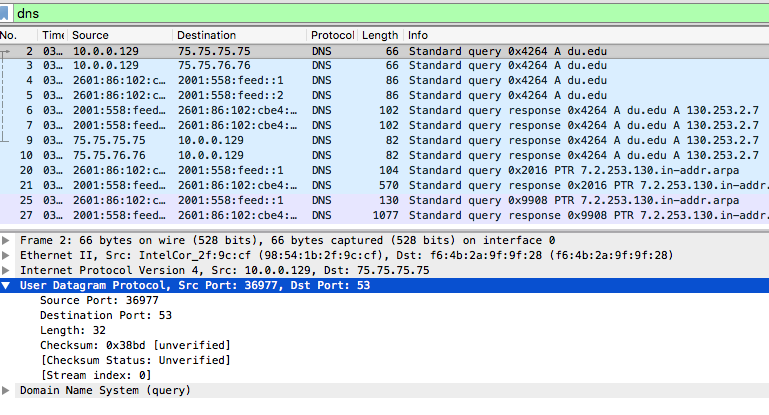
\includegraphics[height = 250pt, keepaspectratio]{Snapshots/q1/1_2.png}
\end{figure}

The port numbers used for sending the packet is $36977$ and receiving the packet is $53$. 

\subsection{:}
- The destination of packet $2$ is $75.75.75.75$. \\
- It is a DNS query of type \textbf{A} as shown. In this, we give the hostname in the query and receive the IPA in the response. 
\\
\begin{figure}[H]
	\vspace{0pt}
	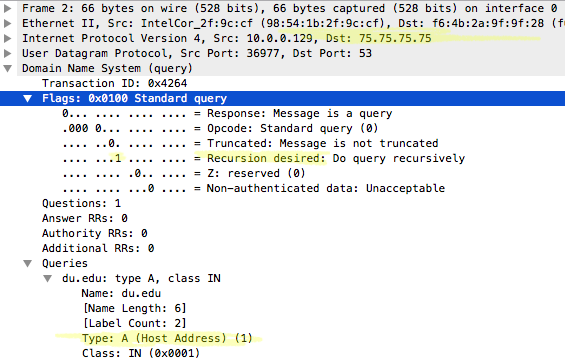
\includegraphics[height = 200pt, keepaspectratio]{Snapshots/q1/1_3_1.png}
\end{figure}
- The only flag set in the query is \textbf{recursion desired}.
\\
- To know the type of DNS server, we check the response to this query. 
\begin{figure}[H]
	\vspace{0pt}
	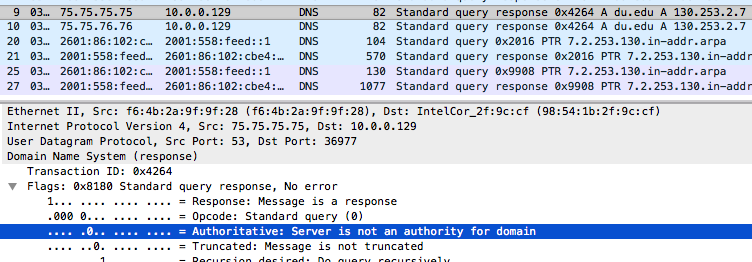
\includegraphics[height = 150pt, keepaspectratio]{Snapshots/q1/1_3_2.png}
\end{figure}
In the response, the flag \textbf{authoritative} is not set. Thus, it must be a local server having the IPA of the hostname cached. 

\subsection{:}

\begin{figure}[H]
	\vspace{0pt}
	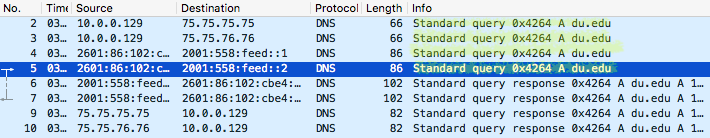
\includegraphics[height = 75pt, keepaspectratio]{Snapshots/q1/1_4.png}
\end{figure}
Total 4 DNS servers are queried for resolving the domain name du.edu.

\subsection{:}

\begin{figure}[H]
	\vspace{0pt}
	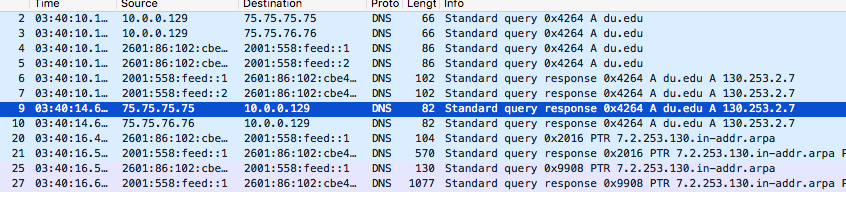
\includegraphics[height = 100pt, keepaspectratio]{Snapshots/q1/1_5_1.png}
\end{figure}

Packet \#9 contains the response of the query sent in packet \#2 as highlighted. The flags set are response, recursion desired and recursion available.

\begin{figure}[H]
	\vspace{0pt}
	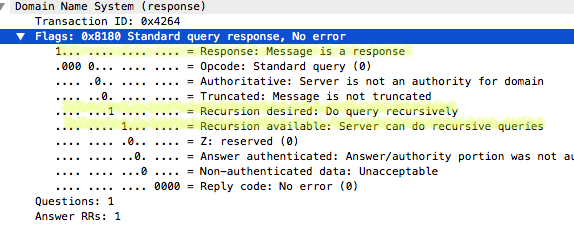
\includegraphics[height = 150pt, keepaspectratio]{Snapshots/q1/1_5_2.png}
\end{figure}

\subsection{:}

\begin{figure}[H]
	\vspace{0pt}
	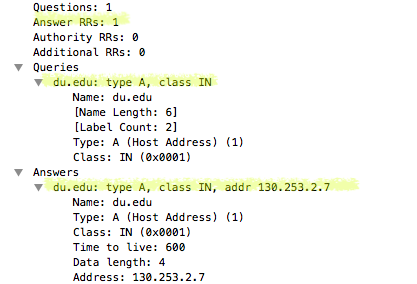
\includegraphics[height = 150pt, keepaspectratio]{Snapshots/q1/1_6_1.png}
\end{figure}

We get one answer from the server. The response is not from an authoritative server as this flag is not set. 

\begin{figure}[H]
	\vspace{0pt}
	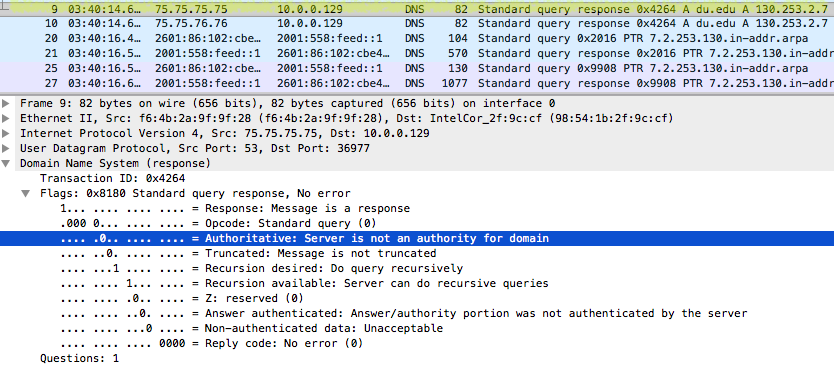
\includegraphics[height = 150pt, keepaspectratio]{Snapshots/q1/1_6_2.png}
\end{figure}

\subsection{:}

\begin{figure}[H]
	\vspace{0pt}
	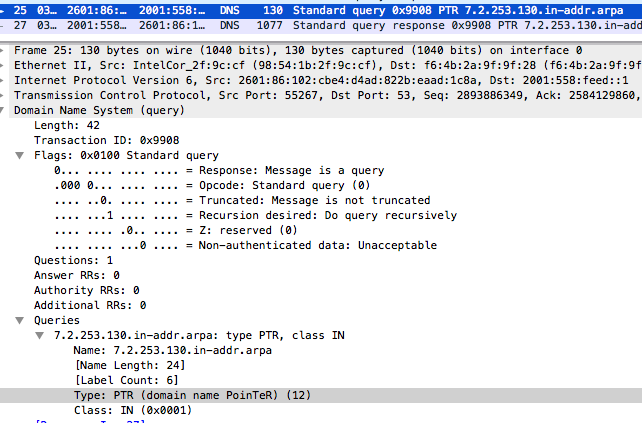
\includegraphics[height = 250pt, keepaspectratio]{Snapshots/q1/1_7.png}
\end{figure}

The query in packet \#25 is of the type PTR and it is used for reverse DNS lookup, i.e. given the IPA, the hostname is provided in the response. 

\subsection{:}

The packet \#27 contains the response of the packet \#25.
\begin{figure}[H]
	\vspace{0pt}
	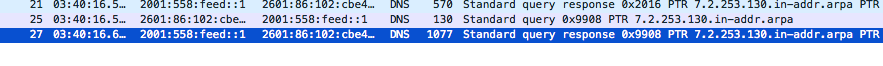
\includegraphics[height = 30pt, keepaspectratio]{Snapshots/q1/1_8_1.png}
\end{figure}

\begin{figure}[H]
	\vspace{0pt}
	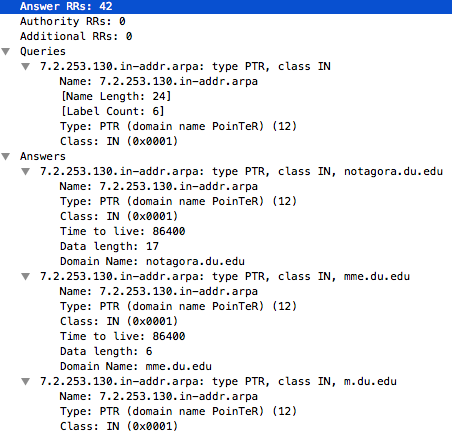
\includegraphics[height = 250pt, keepaspectratio]{Snapshots/q1/1_8_2.png}
\end{figure}
The response contains 42 resource records. All of them contain the hostname to which the queried IPA maps to. 

\section{SET 2: Using the DNS\_2.pcapng:}

\subsection{:}

\begin{figure}[H]
	\vspace{0pt}
	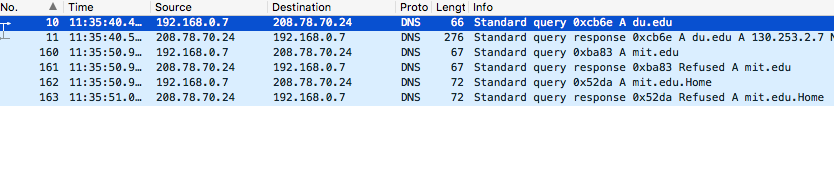
\includegraphics[height = 100pt, keepaspectratio]{Snapshots/q2/2_1_1.png}
\end{figure}

The destination IPA of the server is $208.78.70.24$. 

\begin{figure}[H]
	\vspace{0pt}
	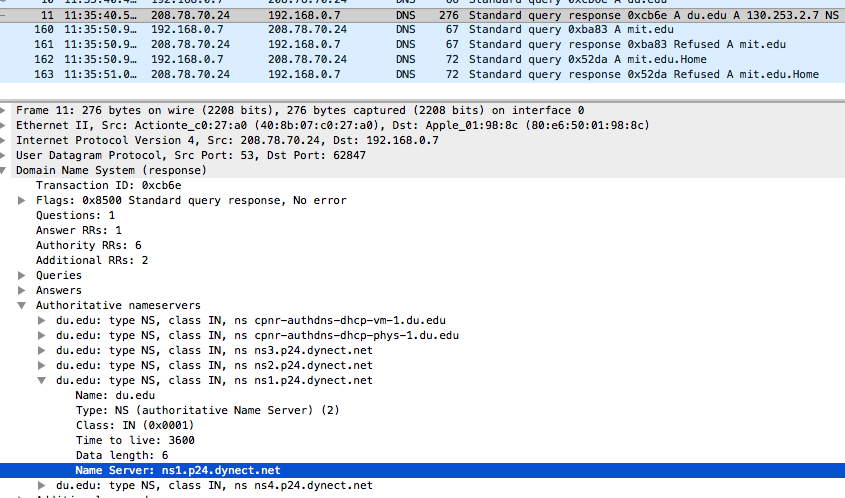
\includegraphics[height = 250pt, keepaspectratio]{Snapshots/q2/2_1_2.png}
\end{figure}

The request is being sent to the authoritative name server \textbf{ns1.p24.dynect.net} as seen in the response in the packet \#11. 

\subsection{:}

\begin{figure}[H]
	\vspace{0pt}
	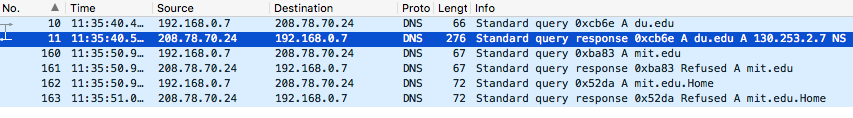
\includegraphics[height = 60pt, keepaspectratio]{Snapshots/q2/2_2_1.png}
\end{figure}

Packet \#11 contains the reply of the query sent in the packet \#10. Yes, the DNS server replied as we are getting a standard query response. 

\begin{figure}[H]
	\vspace{0pt}
	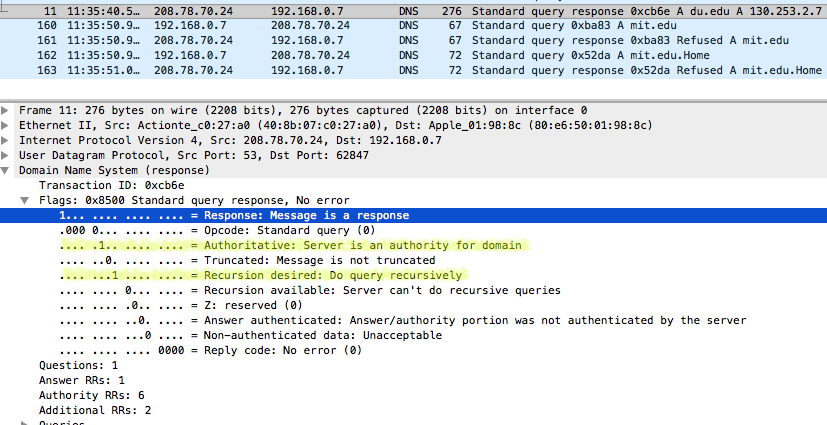
\includegraphics[height = 200pt, keepaspectratio]{Snapshots/q2/2_2_2.png}
\end{figure}

The response, recursion desired and authoritative flags are set in the response. 

\subsection{:}

\begin{figure}[H]
	\vspace{0pt}
	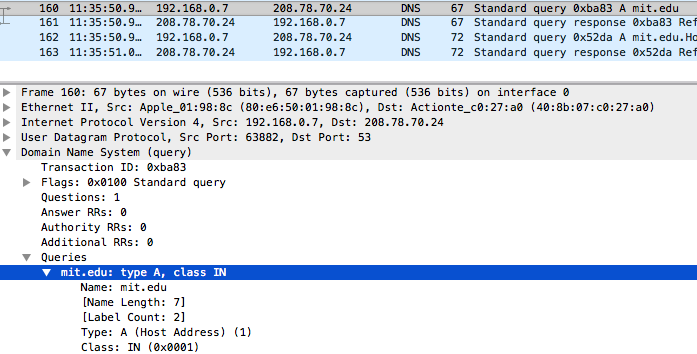
\includegraphics[height = 200pt, keepaspectratio]{Snapshots/q2/2_3.png}
\end{figure}

The DNS request in \#160 is sent to \textbf{ns1.p24.dynect.net}. The DNS request asks the IPA of the hostname \textbf{mit.edu} as the type of query is \textbf{A}.

\subsection{:}

The response from the DNS server for the query sent in packet \#160, as shown in the packet \#161, contains no answer RRs. The reply code is refused. So, the server did not resolve the DNS request. 

\begin{figure}[H]
	\vspace{0pt}
	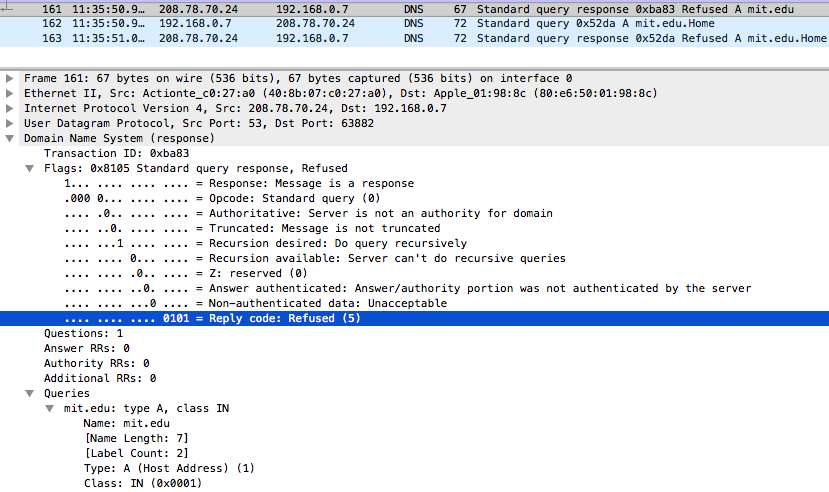
\includegraphics[height = 250pt, keepaspectratio]{Snapshots/q2/2_4.png}
\end{figure}

%%%%%%%%%%%%%%%%%%%%%%%%%%%%%%%%%%%%%%%%%%%%%%%%

\end{document}